\newpage
\section{Figures}
\renewcommand{\thefigure}{\thesection \arabic{figure}}
\setcounter{figure}{0}

\begin{figure}[htbp]
  \centering
  \begin{subfigure}[t]{0.48\linewidth}
    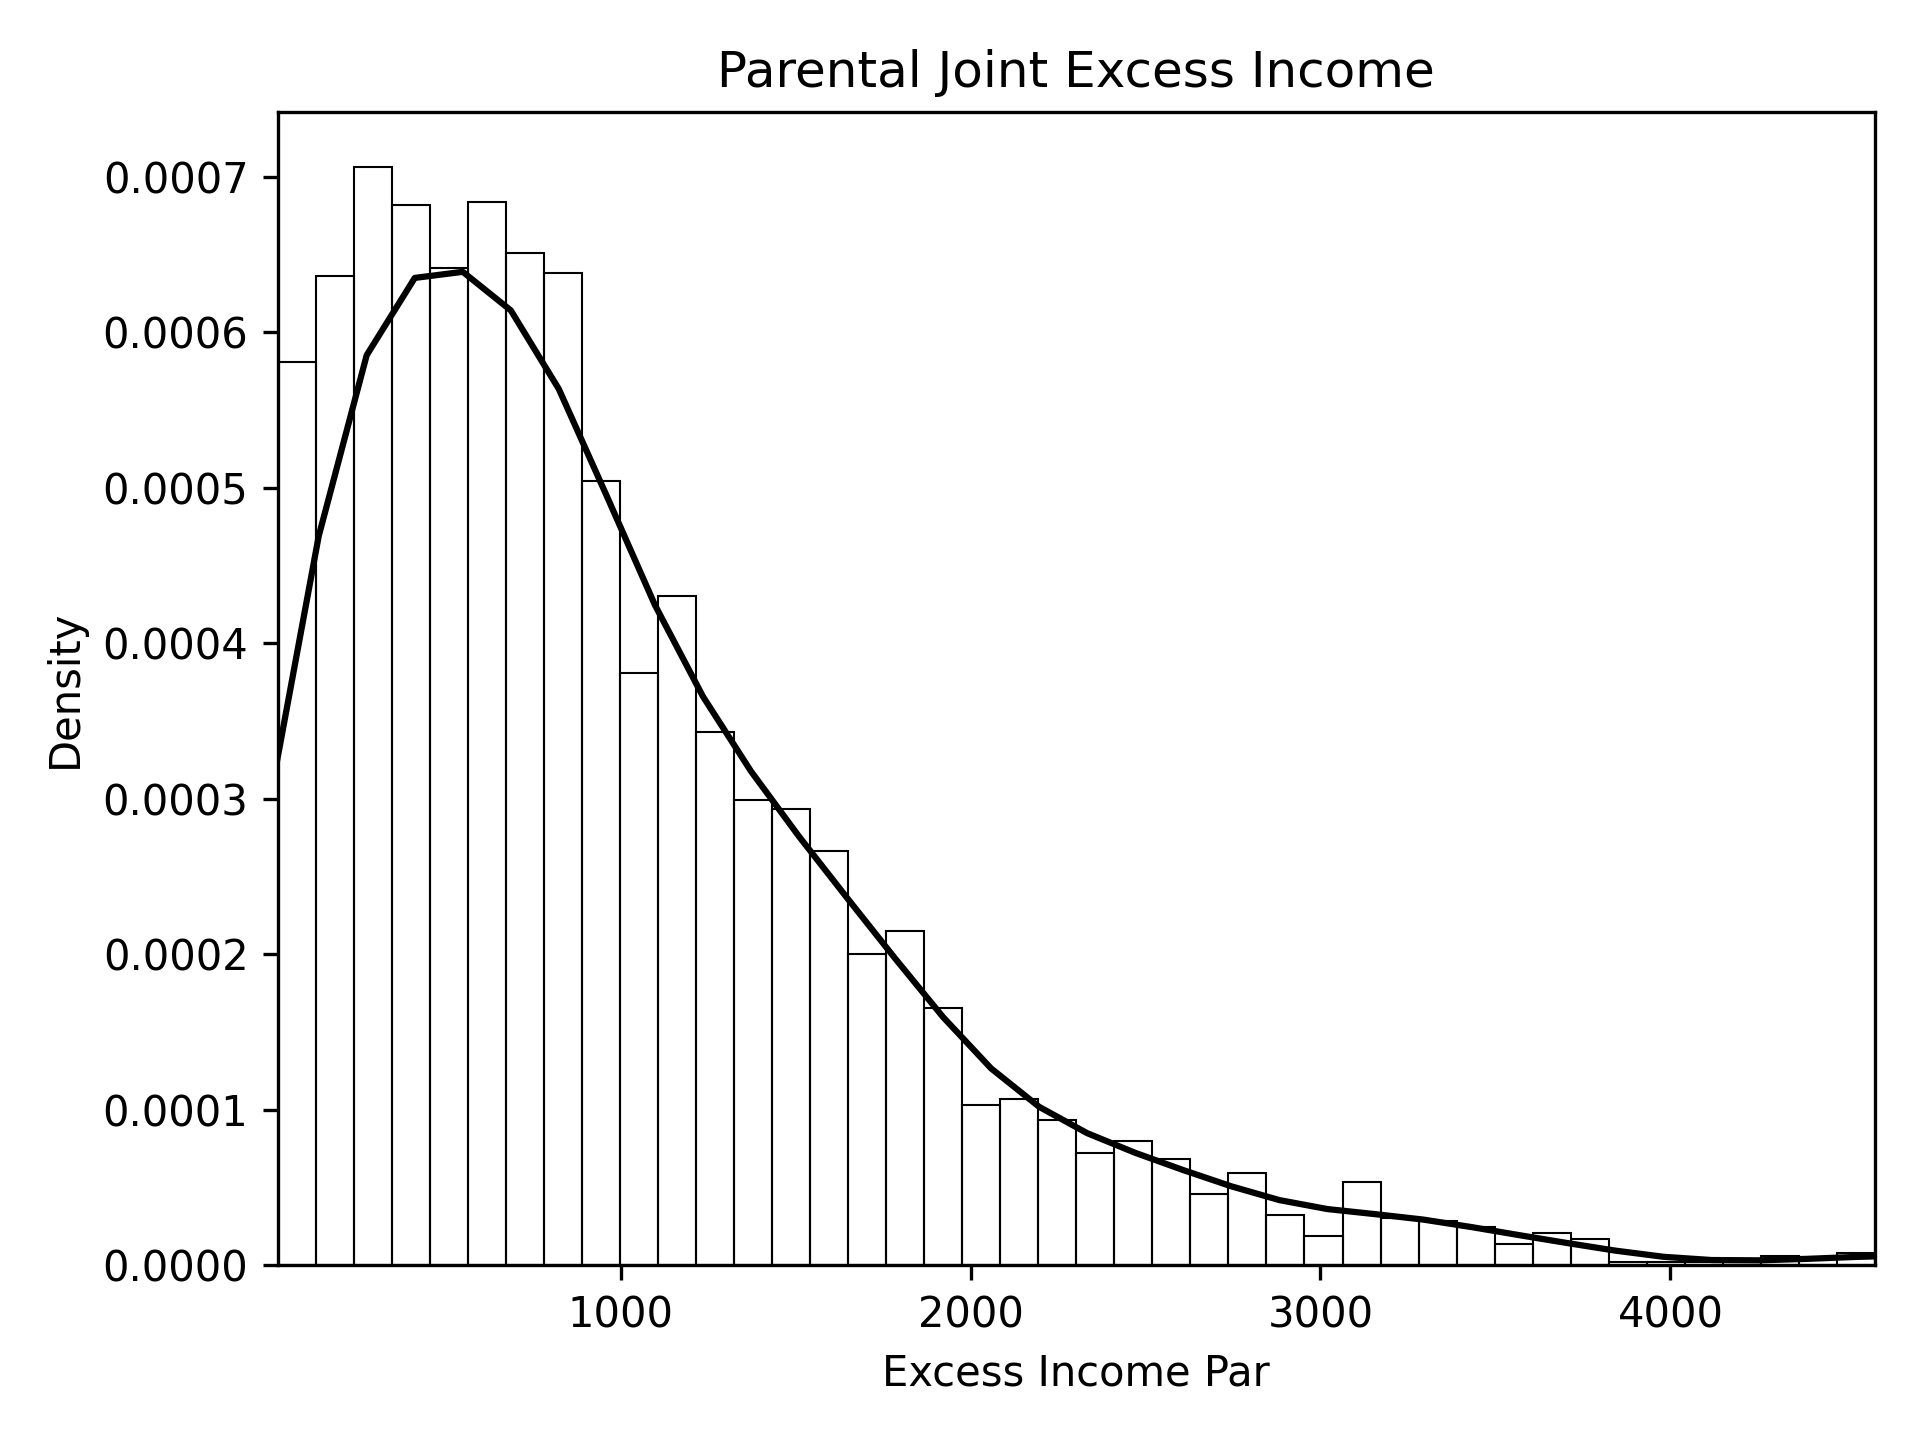
\includegraphics[width=\linewidth]{parental_joint_excess_income_pdf.png}
    \caption{Parental joint excess income}
    \label{fig:parental-excess}
  \end{subfigure}
  \hfill
  \begin{subfigure}[t]{0.48\linewidth}
    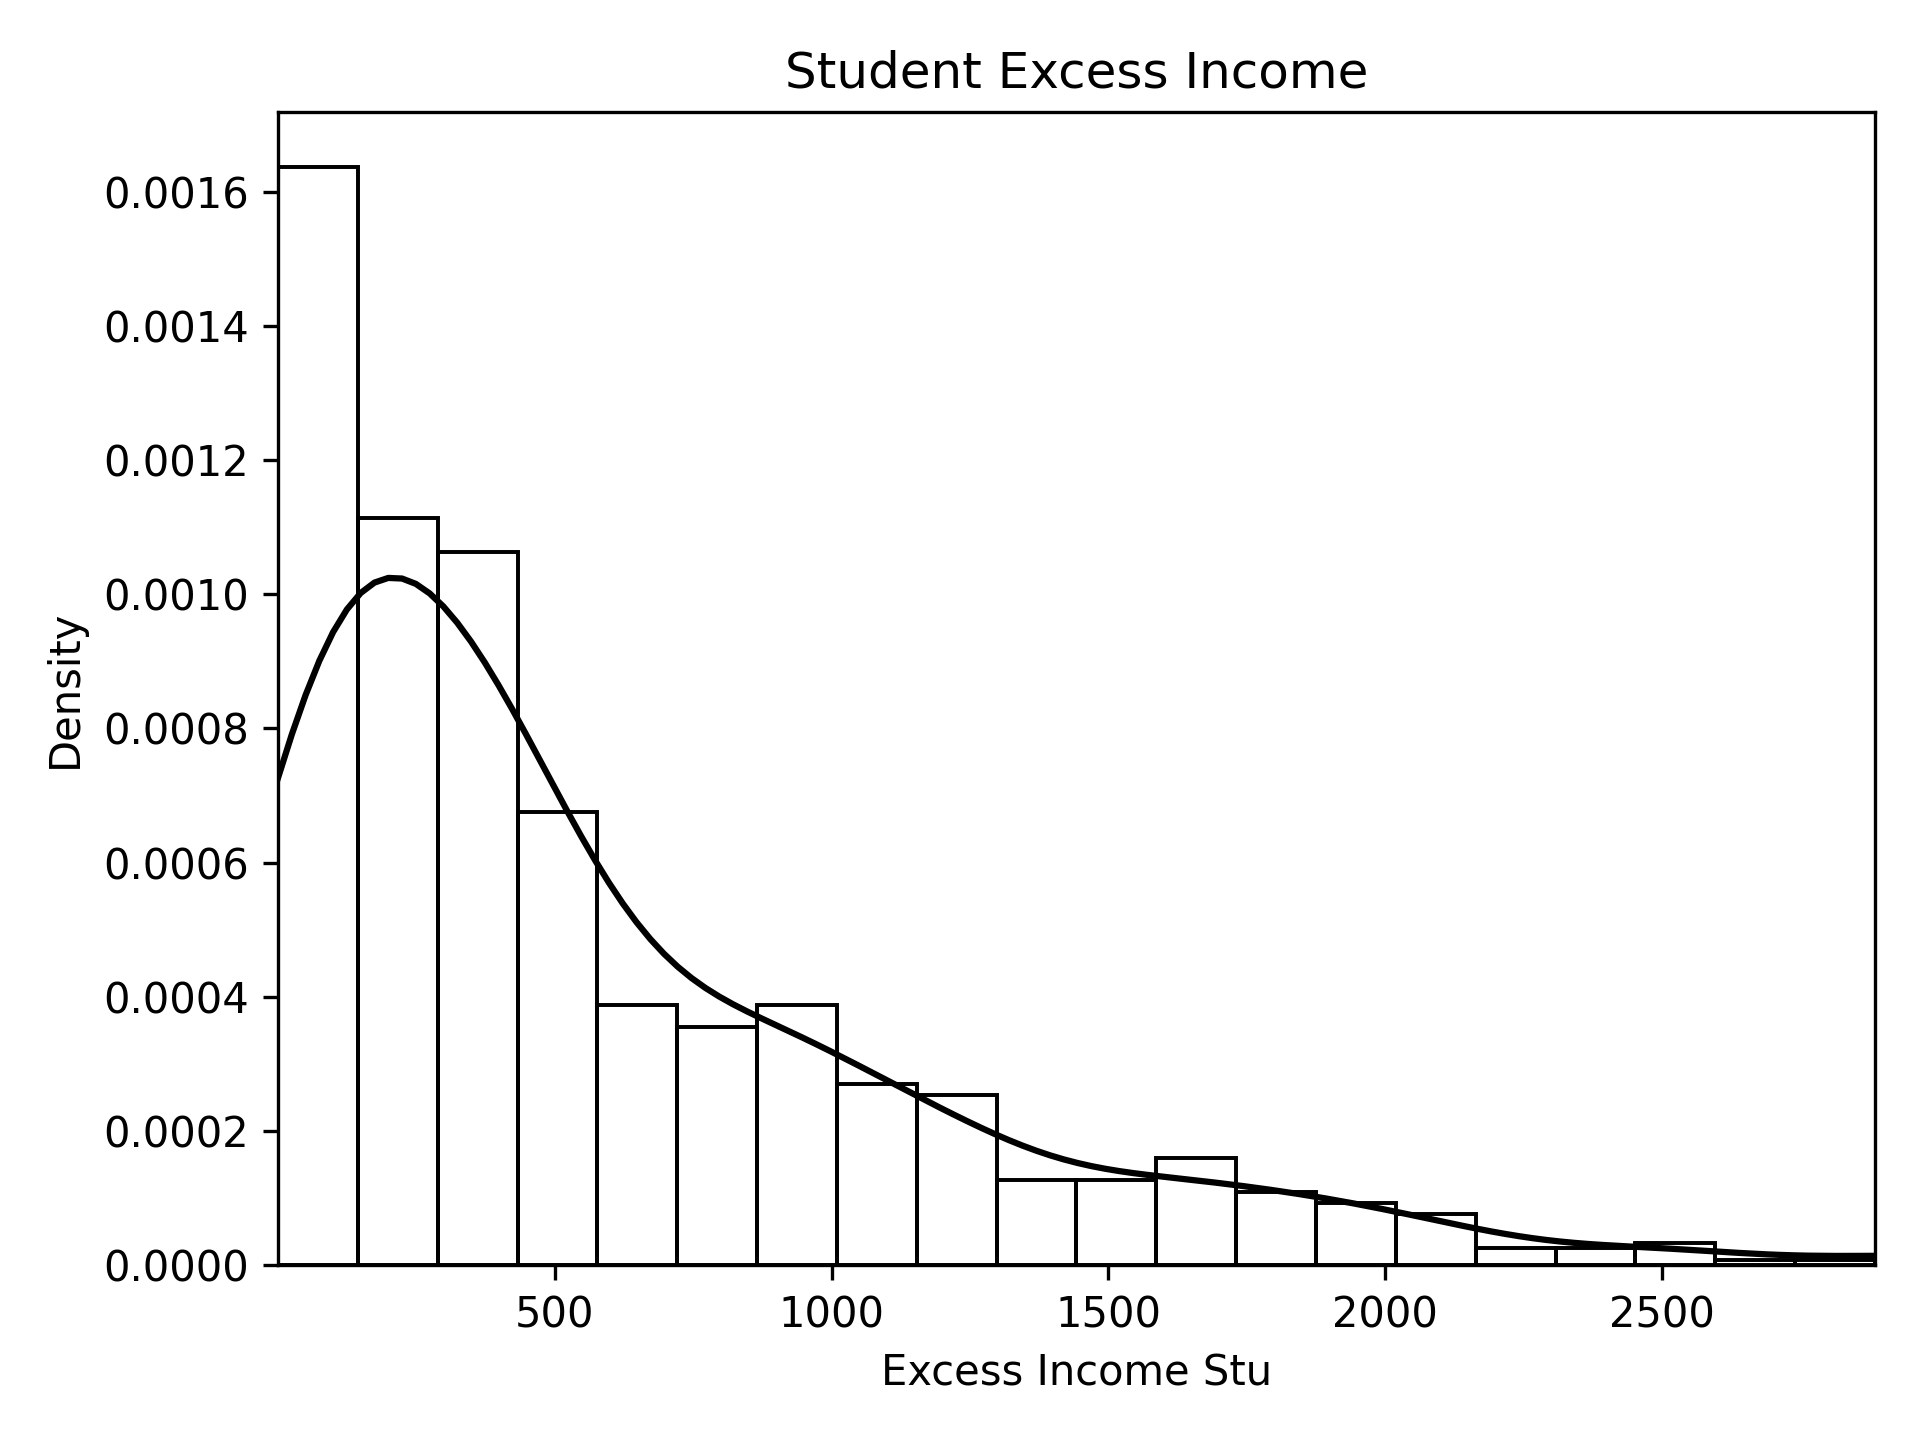
\includegraphics[width=\linewidth]{student_excess_income_pdf.png}
    \caption{Student excess income}
    \label{fig:student-excess}
  \end{subfigure}
  \caption{Simulated mean excess income for parents (\subref{fig:parental-excess}) and students (\subref{fig:student-excess}).}
  \label{fig:excess-income}
\end{figure}


\begin{figure}[htbp]
  \centering
  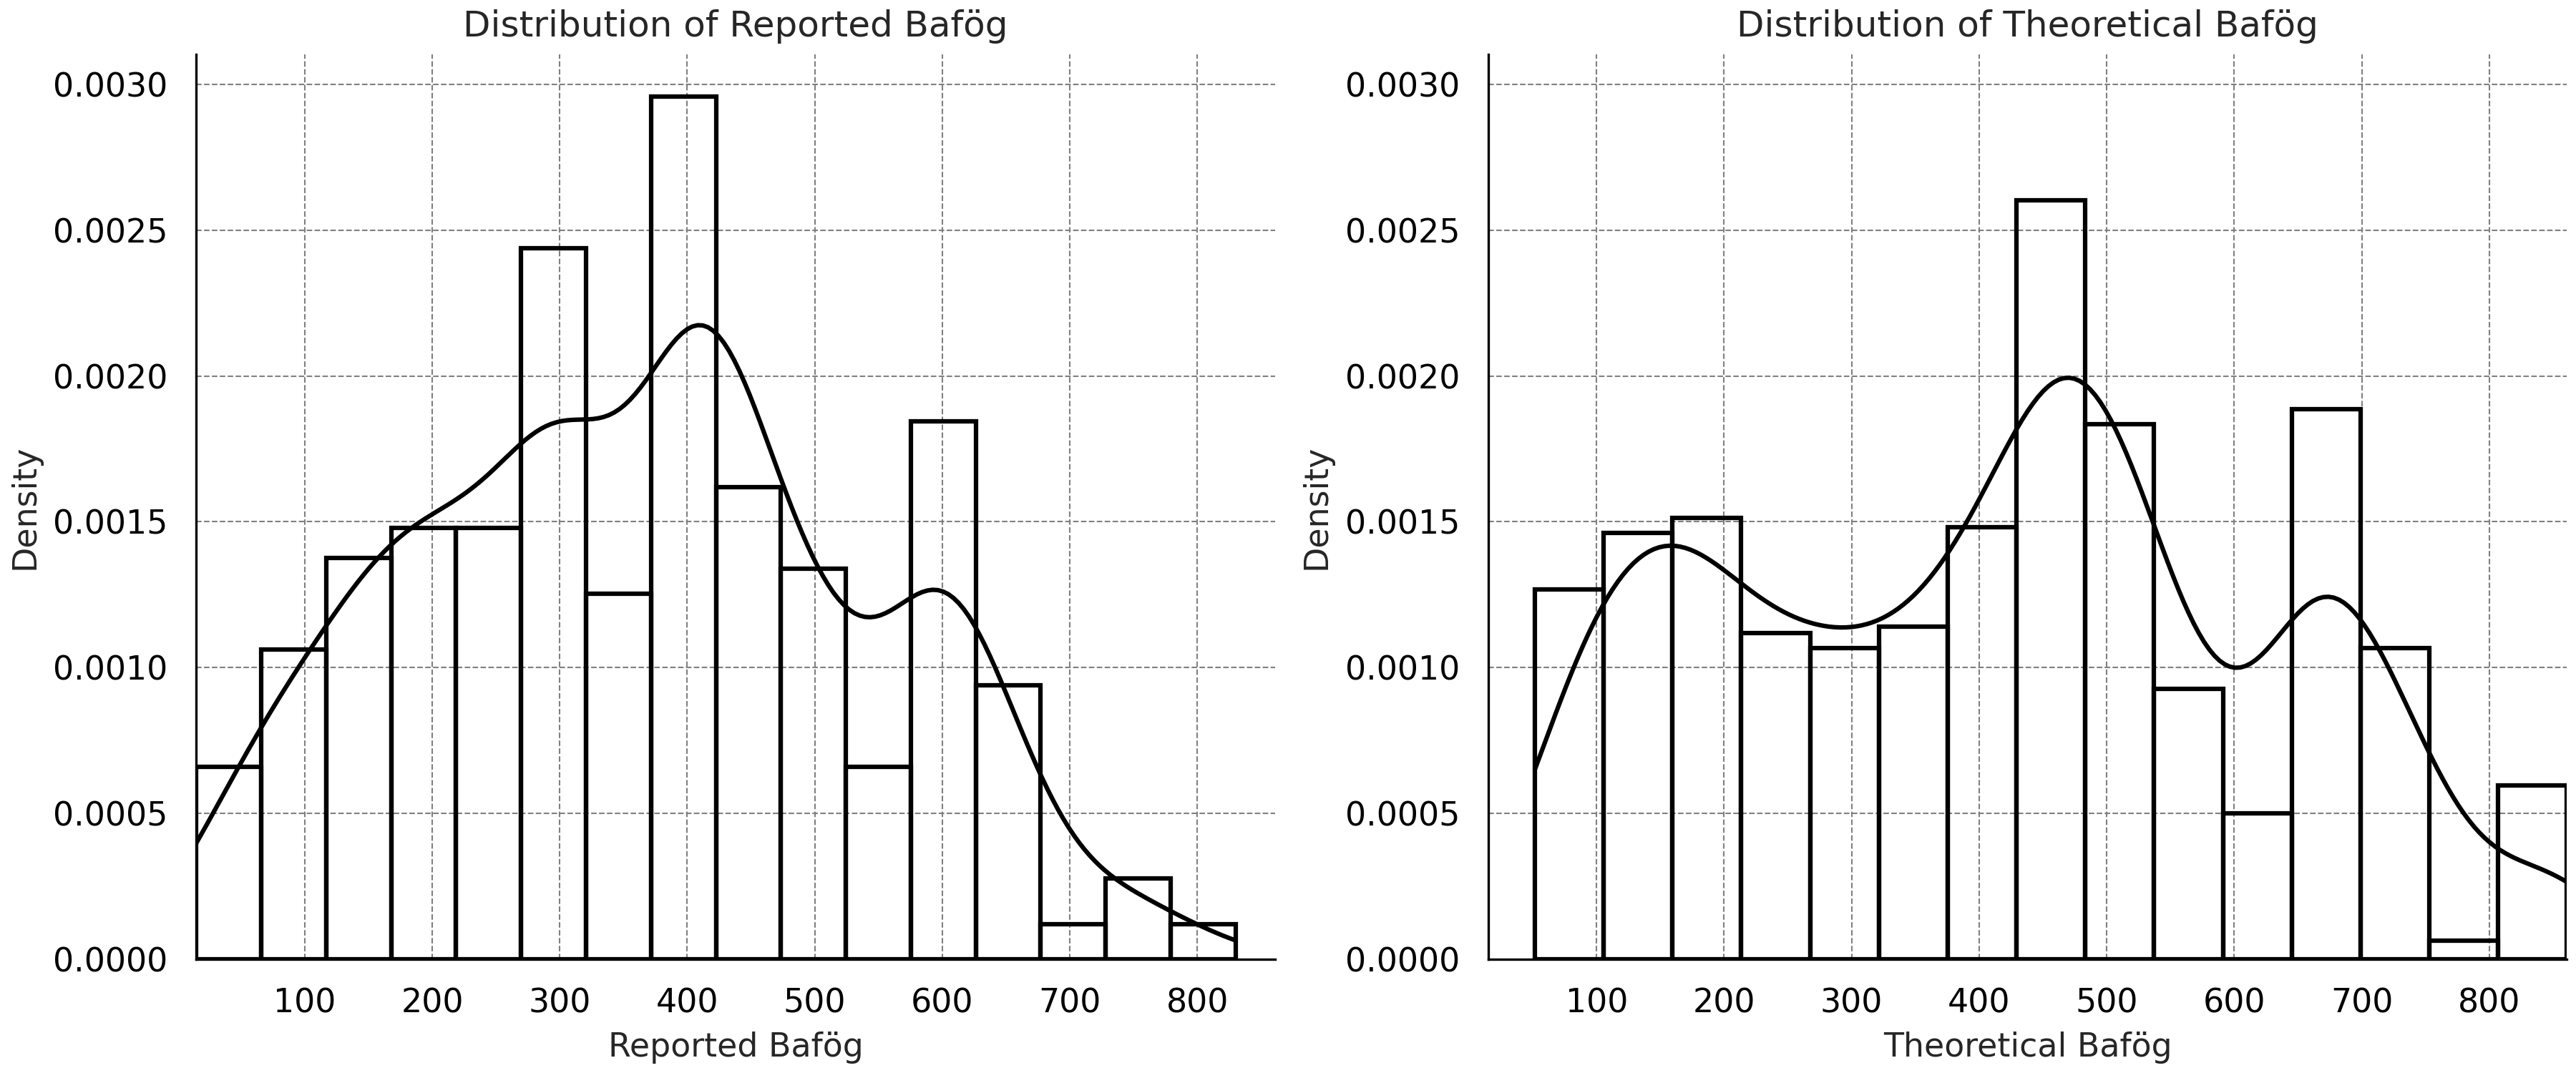
\includegraphics[width=0.95\linewidth]{theo_vs_reported_distribution.png}
  \caption{Comparison of the distribution of reported BAföG receipt in the SOEP-Core sample with the simulated (theoretical) distribution of simulated BAföG entitlements from our model.}
  \label{fig:theo-vs-reported}
\end{figure}


\begin{figure}[H]
  \centering

  \begin{minipage}[t]{0.48\textwidth}
    \centering
    \includegraphics[width=0.95\linewidth]{fraction_of_enrolled_students_receiving_bafog.png}
    \caption{
      Fraction of enrolled students in Germany receiving partial, full, or combined BAföG support (loans and grants). Based on official statistics from Destatis. \textit{Own illustration}.
    }
    \label{figure:bafoeg_support}
  \end{minipage}%
  \hfill
  \begin{minipage}[t]{0.48\textwidth}
    \centering
    \includegraphics[width=0.95\linewidth]{payout_over_time.png}
    \caption{
      Average nominal and real monthly BAföG payout for students (excluding pupils), based on Destatis time series. \textit{Own illustration}.
    }
    \label{figure:payout_over_time}
  \end{minipage}

\end{figure}
